\section{Localisation}
Localisation is the act of a robot finding out where it is. GPS systems are often used to do this in cases where precision is not critical, e.g. GPS navigation. If precision is critical, e.g. for a robot to drive past obstacles without hitting them, GPS is too imprecise. Other techniques must then be used. To do this, robots often have sensors, such as sonars, LIDARs or cameras. 
The localisation algorithms consists of two main parts, movement and measurement. Movement is imprecise, often because of the mechanical system. Measurements contributes with new knowledge and is therefore the part that narrows the decision, of where the robot is, in. The measurements is often also noisy, but usually less noisy than the movements.
Another important thing in localisation is probability. What is the probability of being in a certain position, given the measurement? To calculate this, Bayes rule is used.
\begin{equation}
p(x|z) = \frac{p(z|x)\cdot p(x)}{p(z)}
\end{equation}
Where $\frac{1}{p(z)}$ is the normalizing factor $\eta$.
\begin{equation}
\eta = \frac{1}{p(z)} = \frac{1}{\sum(p(z|x)\cdot p(x))}
\end{equation}
This gives us the expression:
\begin{equation}
p(x|z) = \eta \cdot p(z|x)\cdot p(x)
\end{equation}

\textbf{Eksample:}\\
A robot is in one of the grids in the map. It can detect if it is in a red or green grid. 
\begin{figure}[H]

\includegraphics[scale=1]{billeder/Localisation01.png}
\caption{The map in which the robot lives}
\end{figure}
If the robot is in a green grid, it detects correctly with 75\% chance. If it is in a red grid, it detects correctly with 90\% chance.
If the robot detects green, what is the probability that it is in a green or a red grid?\\
$z = green$\\
$\eta = \frac{1}{sum(p(z|x)\cdot p(x))} = \frac{1}{0.75 \cdot \frac{3}{5} + 0.1 \cdot 2/5} = 2.04$\\\\
$x = green$\\
$p(x) = \frac{3}{5}$\\
$p(x \mid z) = \eta \cdot p(z|x)\cdot p(x) = 2.04 \cdot 0.75 \cdot \frac{3}{5} = 0.918 = 91.8\%$\\\\
$x = red$\\
$p(x) = \frac{2}{5}$\\
$p(x \mid z) = \eta \cdot p(z|x)\cdot p(x) = 2.04 \cdot 0.1 \cdot \frac{2}{5} = 0.082 = 8.2\%$

\subsection{Markov Localisation}
% Localisation_MarkovLocalisation
The purpose of Markov Localisation is to estimate where the robot is located, given its measurements, movements and a map describing the world in which the robot is placed.
Lets say the robot can move along a wall and sense whether if there is a door next to it or not. We place the robot in a world with a wall with 3 doors.
The estimation of the localisation of the robot is called belief and is the probability of being in a given location, given the previous act. At the beginning, the robot will not know where it is, and therefore it will have a uniformly distributed belief.\\ 
Then the robot takes a measurement, and let's say that it measures a door. Now the new belief is the former belief multiplied with the probability of the measurement z given the position x. 
\begin{equation}
bel'(x) = bel(x) \cdot p(z|x)
\label{ML_eq1}
\end{equation}
After this the robot moves. A movement is often noisy and therefore the precision of the belief will fall. This is illustrated by convolving the belief with the motion model. The motion model consists of a mean $\mu$, representing the noise free movement, and a standard deviation $\sigma$, representing the noise. The result of this step can be seen in \ref{ML_fig1:sub3}.
\begin{equation}
bel'(x) = bel(x) \ast norm(\mu,\sigma)
\label{ML_eq2}
\end{equation}
These two steps are now repeated the rest of the lifetime of the robot. Every time the robot senses, it gets more certain of where it is and every time it moves it gets more uncertain. In figure \ref{ML_fig1} two iterations are shown.

\begin{figure}[H]
\centering

\begin{subfigure}[b]{.8\textwidth}
  \centering
  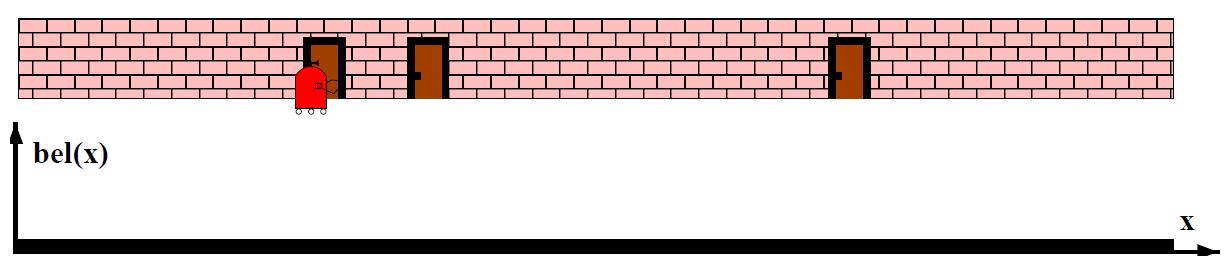
\includegraphics[width=1\linewidth]{billeder/MarkovLocalisation01.png}
  \caption{Initial belief is uniformly distributed.}
  \label{ML_fig1:sub1}
\end{subfigure}%

\begin{subfigure}[b]{.8\textwidth}
  \centering
  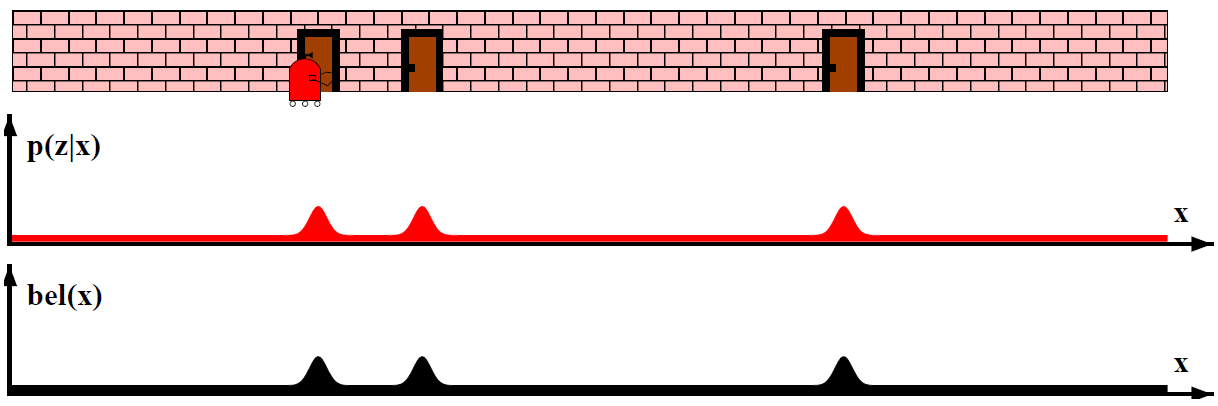
\includegraphics[width=1\linewidth]{billeder/MarkovLocalisation02.png}
  \caption{Measurement and result of belief multiplied with measurement.}
  \label{ML_fig1:sub2}
\end{subfigure}

\begin{subfigure}[b]{.8\textwidth}
  \centering
  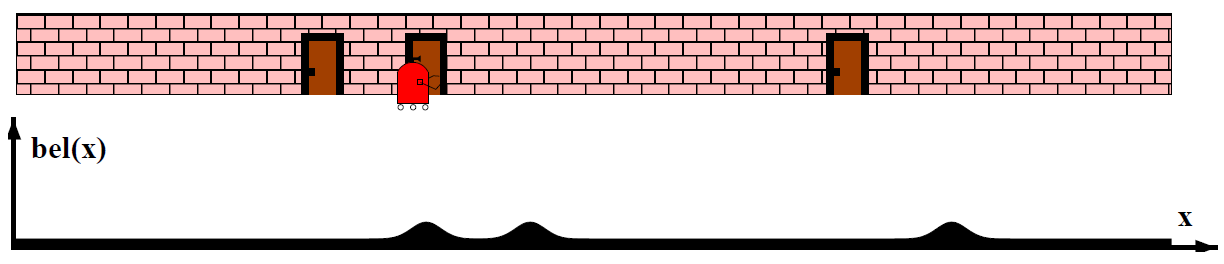
\includegraphics[width=1\linewidth]{billeder/MarkovLocalisation03.png}
  \caption{Movement of robot and belief. Noise makes the belief after the movement more uncertain.}
  \label{ML_fig1:sub3}
\end{subfigure}%

\begin{subfigure}[b]{.8\textwidth}
  \centering
  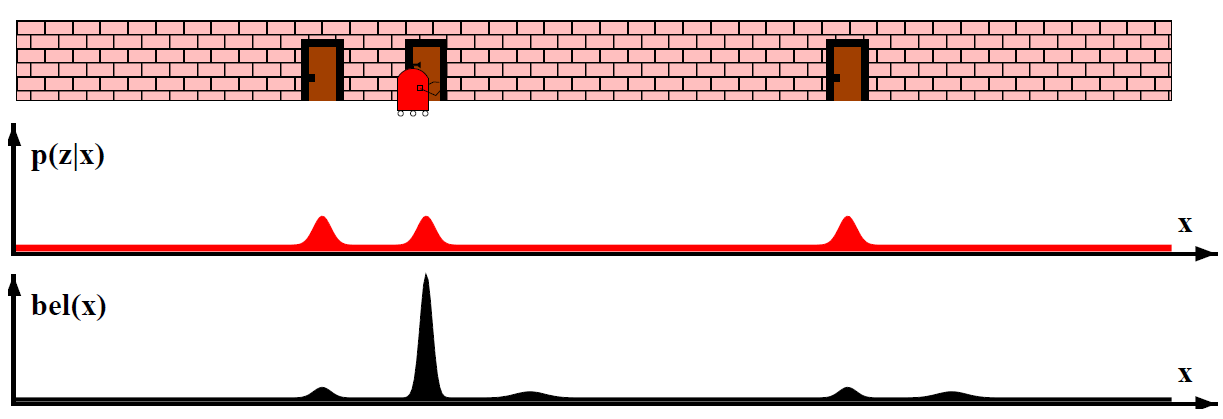
\includegraphics[width=1\linewidth]{billeder/MarkovLocalisation04.png}
  \caption{Measurement and result of belief multiplied with measurement.}
  \label{ML_fig1:sub4}
\end{subfigure}

\begin{subfigure}[b]{.8\textwidth}
  \centering
  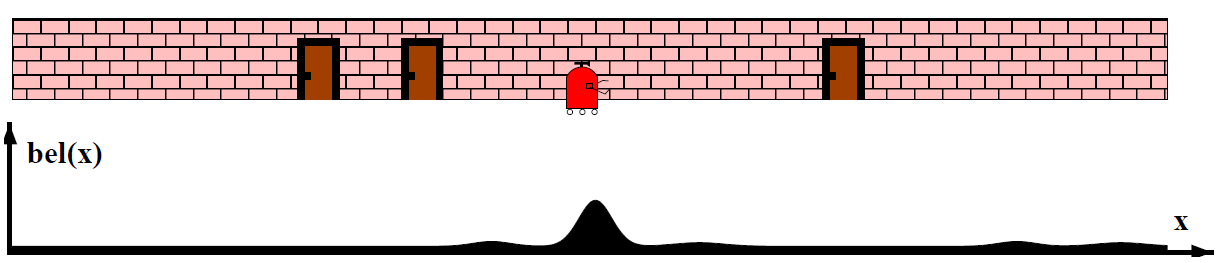
\includegraphics[width=1\linewidth]{billeder/MarkovLocalisation05.png}
  \caption{Movement of robot and belief. Noise makes the belief after the movement more uncertain.}
  \label{ML_fig1:sub5}
\end{subfigure}

\caption{Markov Localisation illustrated. \citep{thrun2005probabilistic}}
\label{ML_fig1}
\end{figure}

The algorithm for Markov Localisation is as follows:\\
1:\quad \textbf{Algorithm MarkovLocalization(}$bel(x_{t-1}),u_t,z_t,m$\textbf{):}\\
2:\quad \quad $for\,all\,x_t\,do$\\
3:\quad \qquad $\overline{bel}(x_t) = \int p(x_t|u_t,x_{t-1},m)\cdot bel(x_{t-1}) dx$\\
4:\quad \qquad $bel(x_t) = \eta p(z_t|x_t,m)\cdot \overline{bel}(x_t)$\\
5:\quad \quad $endfor$\\
6:\quad \quad $return\,bel(x_t)$

What happens is that after a move, $u_t$, and a measurement, $z_t$, has been taken, the algorithm is called. First it calculates the belief after the movement, and then it calculates the belief after the measurement. It does this for all possible places, $x_t$, in the map, $m$. This corresponds to the combinations of (a and b) or (c and d) in figure \ref{ML_fig1}.

\subsection{Kalman Filter}
\lipsum[7] % Dummy text

\subsection{Particle Filter}
\lipsum[7] % Dummy text
%------------------------------------------------